\documentclass{article}
\usepackage{graphicx}

\author{Setsuna}
\title{ECE 60827 CUDA Assignment 1 Report}

\begin{document}
\maketitle
Runtime breakdown of significant components for different vector sizes for SAXPY are reported in figure \ref{fig:p1}.

\begin{figure}[h!]
	\centering
	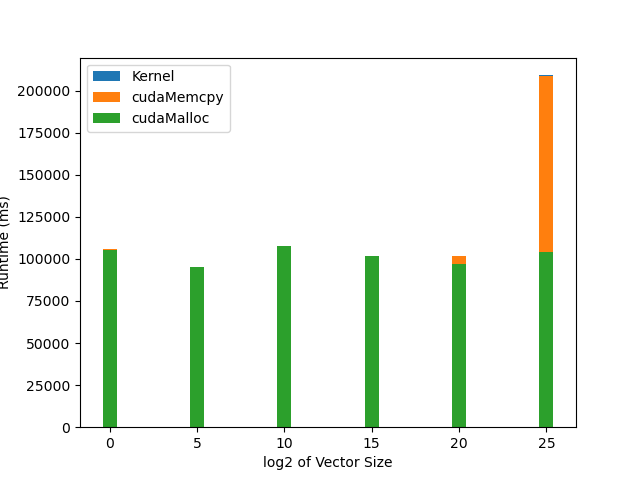
\includegraphics[width=\linewidth]{p1.png}
	\caption{Runtime of SAXPY with different vector size}
	\label{fig:p1}
\end{figure}

Runtime breakdown when varying the number of points in $\pi$ estimator is reported in figure \ref{fig:p2-1}. Varying the number of threads yields runtime result figure \ref{fig:p2-2}.

\begin{figure}[h!]
	\centering
	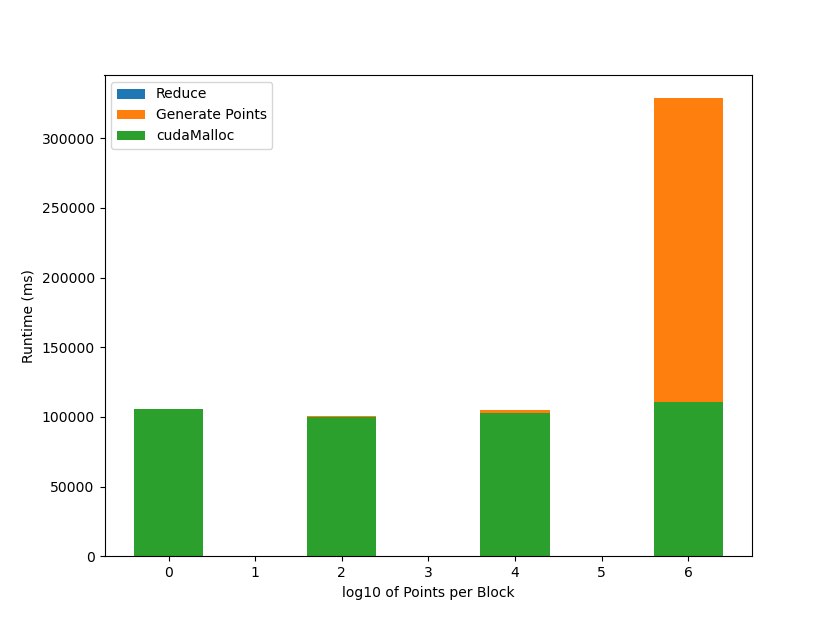
\includegraphics[width=.8\linewidth]{p2-1.png}
	\caption{Runtime of Pi Estimate with different number of points per thread}
	\label{fig:p2-1}
\end{figure}
\begin{figure}[h!]
	\centering
	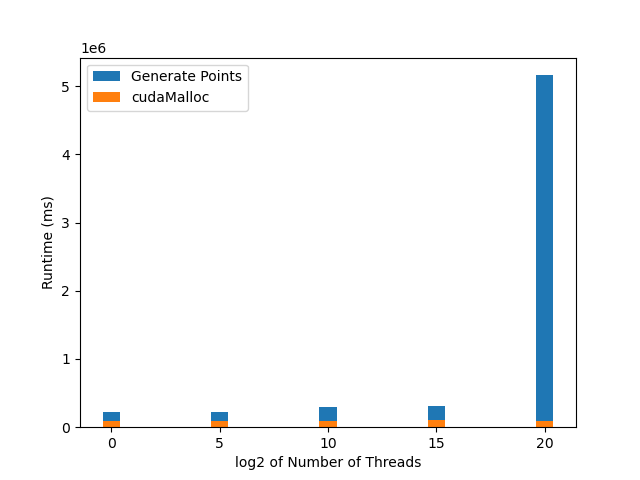
\includegraphics[width=.8\linewidth]{p2-2.png}
	\caption{Runtime of Pi Estimate with different number of threads}
	\label{fig:p2-2}
\end{figure}

Only significant API calls are reported in the breakdown.

As seen in all figures, the runtime of cudaMalloc() stays relatively constant regardless of the amount of data, and is significant especially when the amount of work is small. As expected, when the amount of data increases beyond a certain saturating point, the cudaMemcpy() overhead becomes much more significant. Similar saturating effects are also observed when increasing the number of threads or the amount of work for each thread.

\end{document}